\section*{WRITING TASK 1}
You should spend about 20 minutes on this task.

\begin{quote}\large The diagram shows the main components of a solar-powered ventilation unit and how air moves through it.
\end{quote}
Describe the main features of the information, select relevant details, and make comparisons where appropriate.

\begin{center}
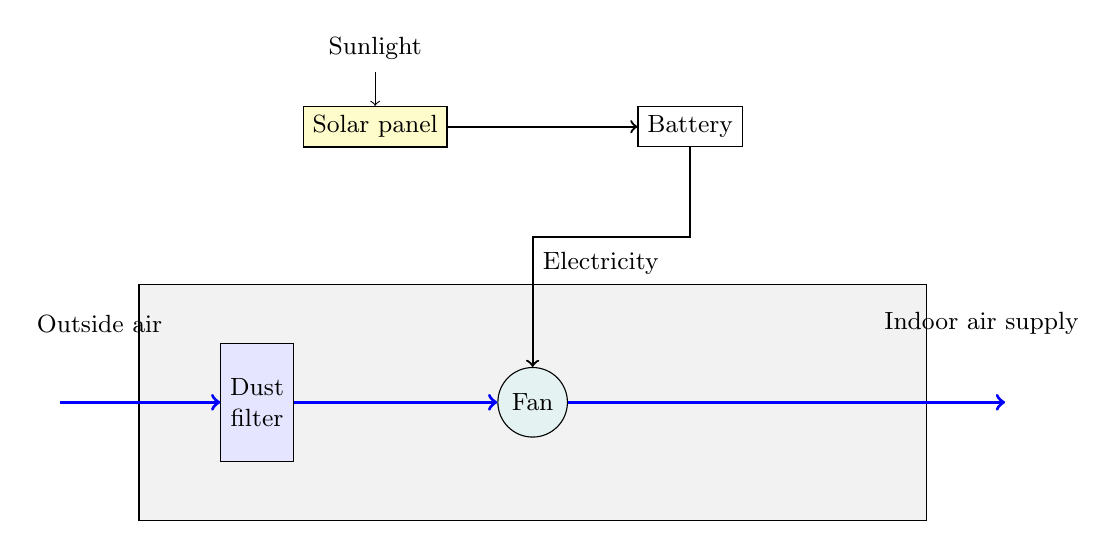
\begin{tikzpicture}[every node/.style={font=\small,align=center}]
\draw[fill=gray!10] (0,0) rectangle (10,3);
\node[draw,fill=blue!10,minimum height=1.5cm] (filter) at (1.5,1.5){Dust\\filter};
\node[draw,circle,fill=teal!10] (fan) at (5,1.5){Fan};
\draw[->,very thick,blue] (-1,1.5)--(filter);\node at (-0.5,2.5){Outside air};
\draw[->,very thick,blue] (filter)--(fan);\draw[->,very thick,blue] (fan)--(11,1.5);\node at (10.7,2.5){Indoor air supply};
\node[draw,fill=yellow!20] (solar) at (3,5){Solar panel};\node[draw] (battery) at (7,5){Battery};
\draw[->,thick] (solar)--(battery);\draw[->,thick] (battery)--(7,3.6)--(5,3.6)--(fan) node[pos=0.2,right]{Electricity};
\node at (3,6){Sunlight};\draw[->] (3,5.7)--(solar);
\end{tikzpicture}
\end{center}
Write at least 150 words.
\par\bigskip
{\footnotesize\color{gray} Original practice material; fictional settings and data. Not an official IELTS examination paper.}
